
\section{Introduction}

This chapter presents the experimental results of the project.
It discusses the main findings obtained from exploratory data analysis, model training, comparative evaluation, and forecasting.
It also highlights the limitations of the current work and proposes directions for improvement.

\section{Exploratory Findings}

The exploratory analysis revealed that the dataset contains meaningful temporal variation and several potentially informative economic indicators.
The evolution of the housing-related target variable suggested long-term trends as well as period-specific changes.

Correlation analysis showed that some macroeconomic variables are more strongly related to the target than others.
However, correlation alone is not sufficient for prediction, especially when variables interact or when relationships are not purely linear.

Distribution plots by administration also suggested that some economic periods differ more clearly than others.
This supports the idea that contextual or policy-related factors may influence the structure of the housing market.

\section{Model Performance}

The final application compares several regression models under the same chronological train-test logic.
This is more reliable than presenting only one model, because the housing dataset contains strong temporal structure and engineered variables such as lagged values and rolling indicators.
The reproducible evaluation generated from the included CSV is presented later in this chapter in Table~\ref{tab:generated_model_metrics}.

In the generated run, Linear Regression obtains the strongest test result because the dataset includes lagged and smoothed price variables that preserve the main direction of the trend.
This does not mean that Linear Regression is always the best model for housing analysis.
It means that, for this specific feature set, a transparent trend-following model generalizes better to the final chronological period than tree-based models.
The Random Forest and Gradient Boosting results remain useful diagnostic evidence because they show the difficulty of extrapolating a rising market when the test period moves outside the range learned in training.

\section{Feature Importance and Interpretation}

The correlation and diagnostic graphics show that lagged and smoothed price indicators are the strongest predictors in the current dataset.
This is coherent with the housing-market context because home prices usually evolve gradually rather than changing abruptly from one month to the next.
Macroeconomic indicators such as mortgage rates, interest rates, inflation, unemployment, income, building permits, and consumer sentiment remain important for interpretation because they explain the market environment around the price movement.

The main lesson is that predictive strength and economic explanation are not identical.
Lag features may predict very well, but the paper-review and OLAP sections are still needed to explain why the market behaves that way.

\section{Forecast Results}

The forecasting component generated a sequence of future estimated values over a selected horizon.
The projected series remained consistent with the historical trajectory and reflected the persistence captured through lag features.

The forecast should be interpreted carefully.
It is not a guarantee of future market behavior.
Instead, it is a model-based projection under the assumptions embedded in the training data and the chosen feature engineering process.

\section{Dashboard Contribution}

Beyond the numerical metrics, the dashboard is one of the most valuable outcomes of the project.
It transforms the analysis into an interactive environment where users can:
\begin{itemize}
\item inspect data quality,
\item select targets and features,
\item compare periods,
\item visualize distributions,
\item train models,
\item and export results.
\end{itemize}

This practical dimension increases the usefulness of the project and makes the results easier to communicate.

\section{Data-Driven Result Snapshot}

To make the final discussion concrete, the report assets were regenerated from the included CSV file using a chronological 80/20 train-test split. The target variable is \texttt{Home\_Price\_Index}, and the predictors are the remaining numerical macroeconomic and engineered features. This makes the reported results reproducible from the project package.

\begin{figure}[H]
\centering
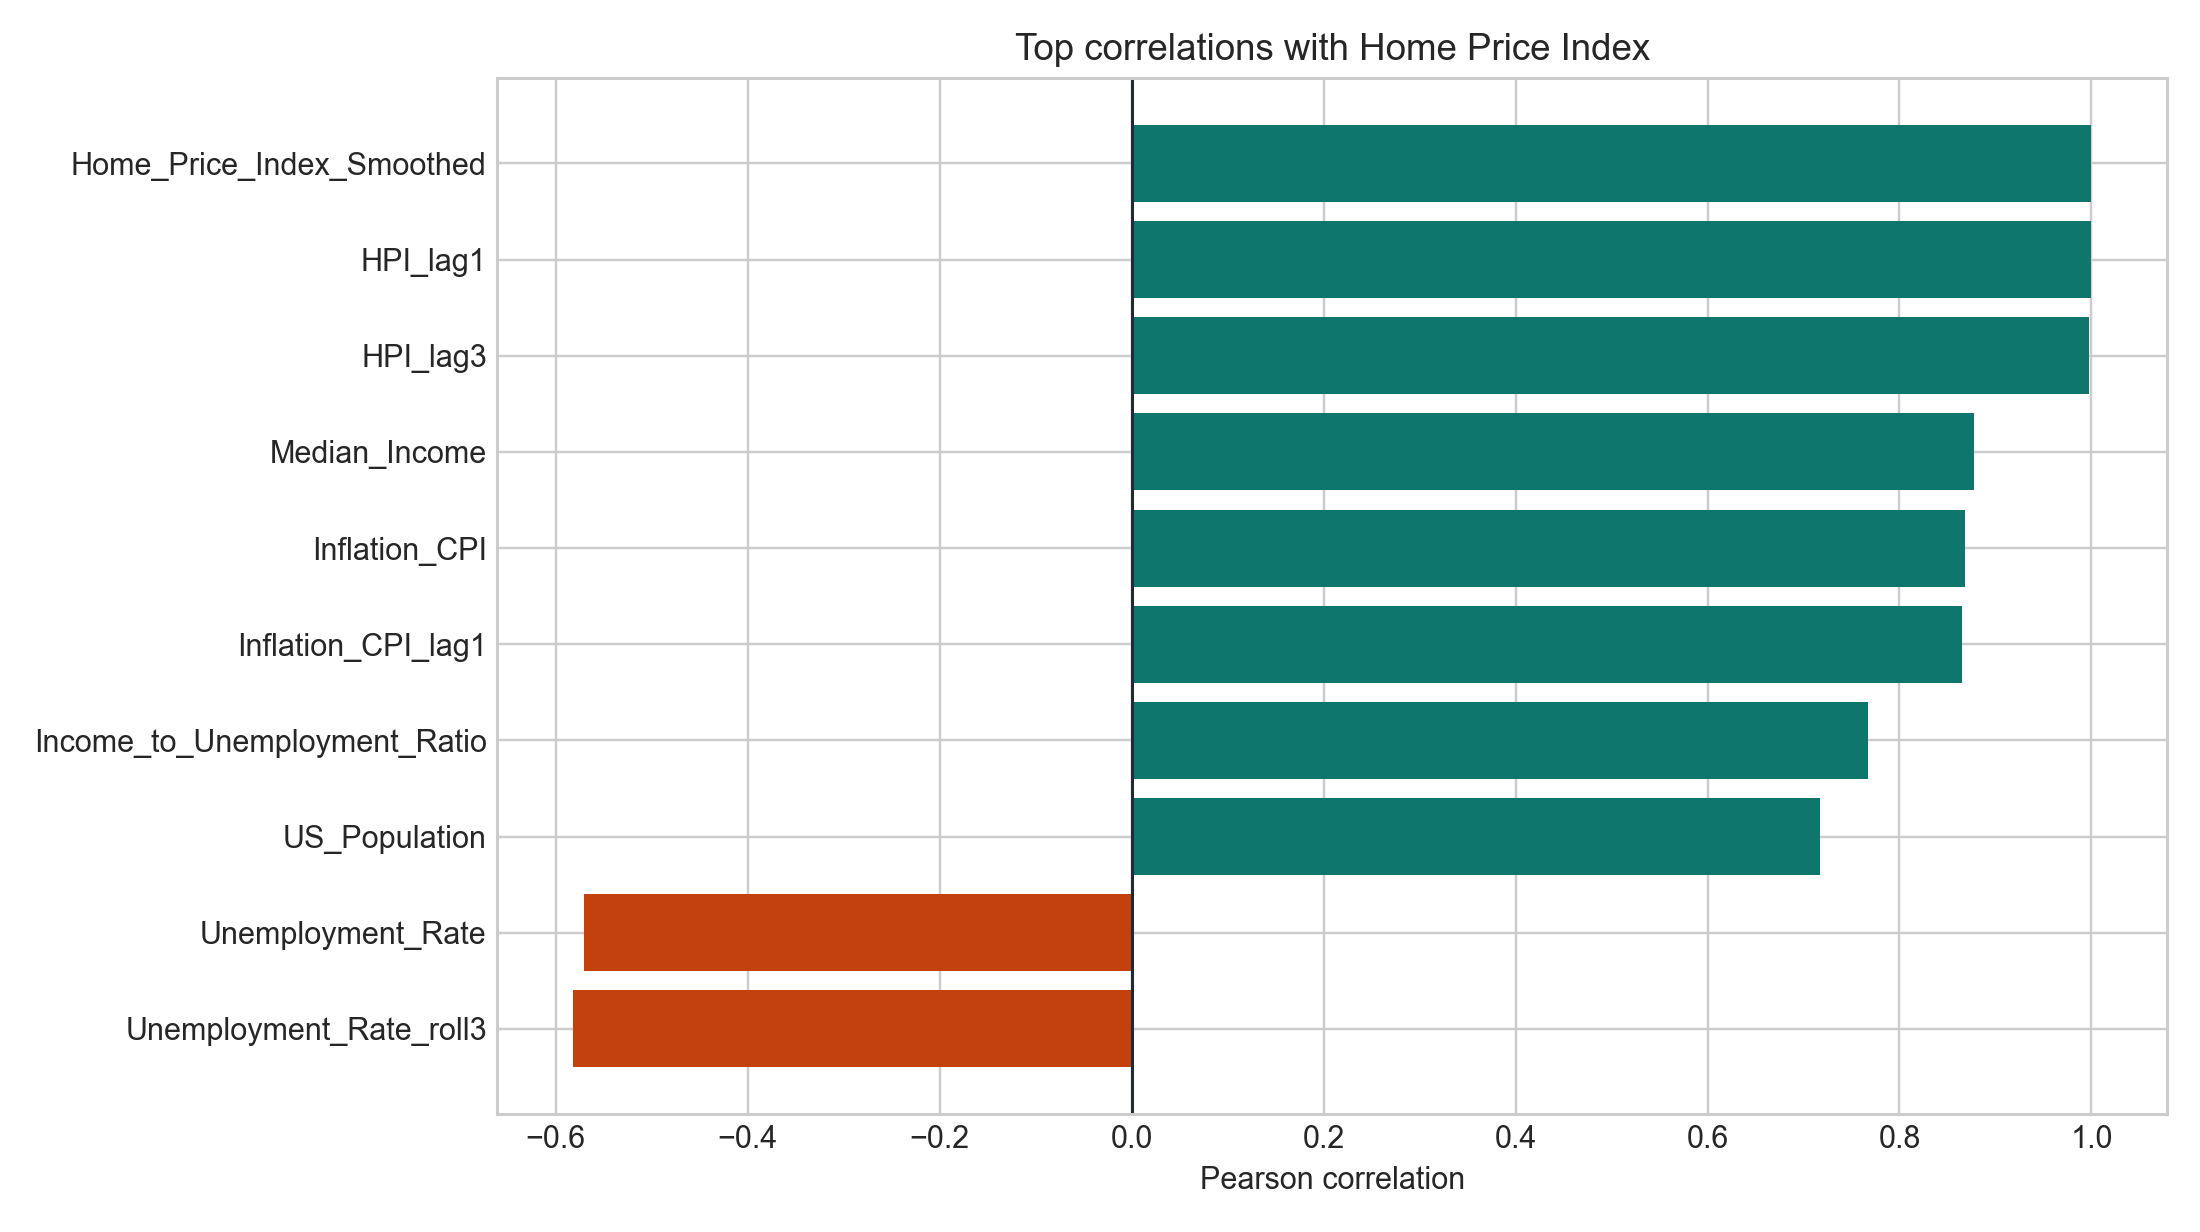
\includegraphics[width=0.92\textwidth]{figures/correlation_results.png}
\caption{Strongest correlations with the Home Price Index in the project dataset.}
\label{fig:generated_corr}
\end{figure}

The strongest linear relationships with the target are: \texttt{Home\_Price\_Index\_Smoothed} (1.00), \texttt{HPI\_lag1} (1.00), \texttt{HPI\_lag3} (1.00), \texttt{Median\_Income} (0.88). These correlations support the paper-review conclusion that housing prices should be interpreted through several linked economic forces, not through a single variable.

\begin{table}[H]
\centering
\begin{tabular}{lrrrr}
\toprule
\textbf{Model} & \textbf{MAE} & \textbf{RMSE} & \textbf{$R^2$} & \textbf{CV $R^2$} \\
\midrule
Linear Regression & 0.661 & 0.797 & 0.999 & 0.994 \\
Ridge Regression & 3.715 & 4.162 & 0.984 & -3.135 \\
Gradient Boosting & 65.816 & 73.669 & -4.148 & -2.458 \\
Decision Tree & 66.218 & 73.750 & -4.159 & -3.315 \\
Random Forest & 69.077 & 76.105 & -4.494 & -2.619 \\
KNN & 74.459 & 79.883 & -5.053 & -4.314 \\
SVR & 103.767 & 109.606 & -10.395 & -7.678 \\
\bottomrule
\end{tabular}
\caption{Generated regression comparison on the chronological test set.}
\label{tab:generated_model_metrics}
\end{table}

The best test-set model in this generated run is \textbf{Linear Regression}, with \(R^2=0.999\), RMSE \(=0.797\), and MAE \(=0.661\). Because the dataset includes lagged and smoothed price features, the linear model can extrapolate the rising trend very effectively. The weaker tree-model scores are also informative: tree ensembles can capture non-linear interactions, but they may struggle when the test period moves beyond the range learned during training.

\begin{figure}[H]
\centering
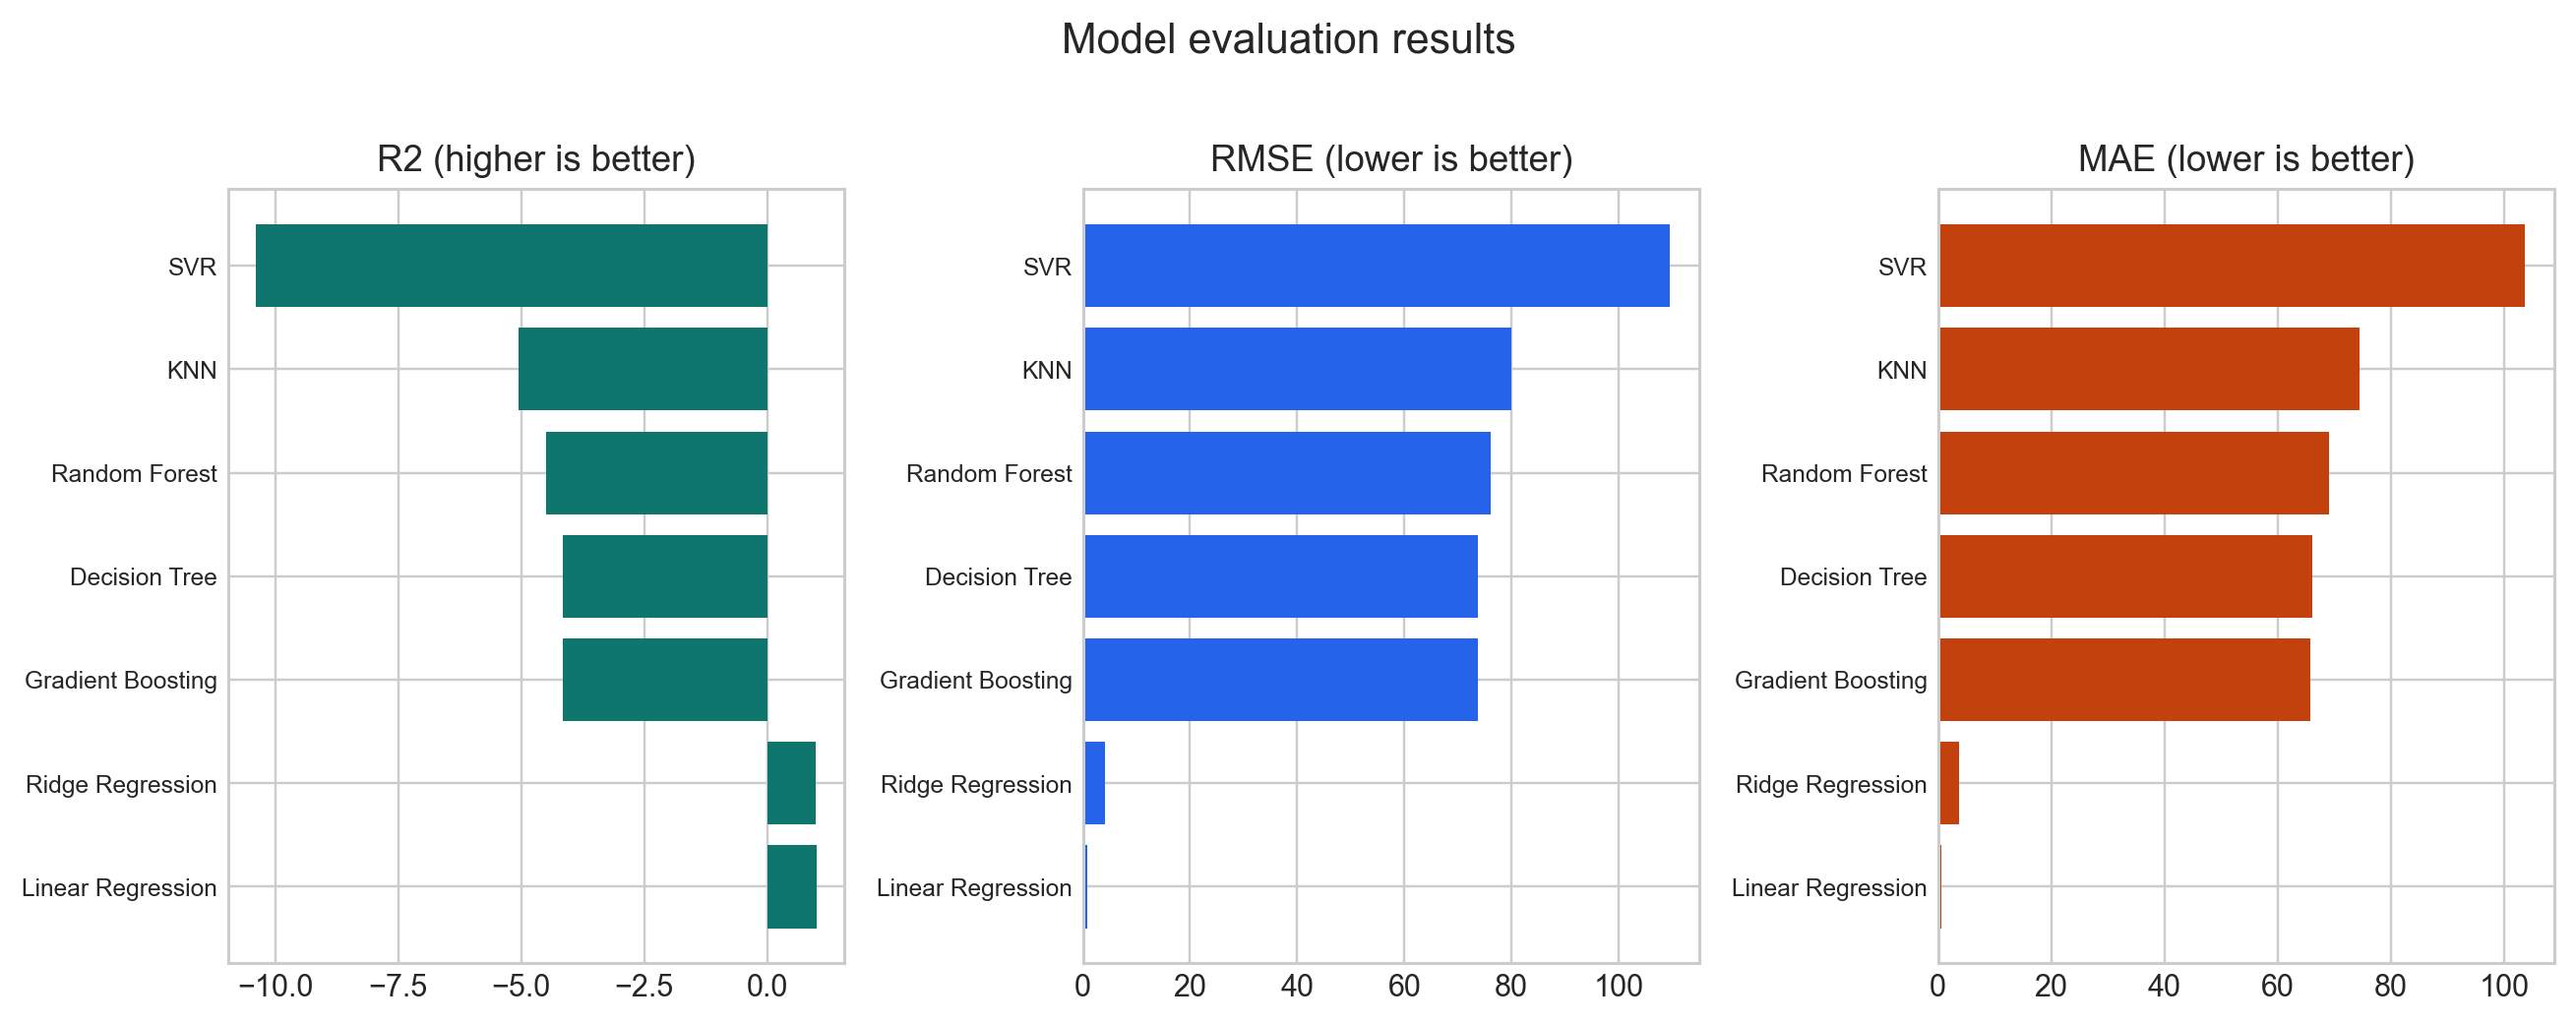
\includegraphics[width=0.98\textwidth]{figures/model_evaluation_results.png}
\caption{Evaluation graphics generated from the model comparison module.}
\label{fig:generated_eval}
\end{figure}

\begin{figure}[H]
\centering
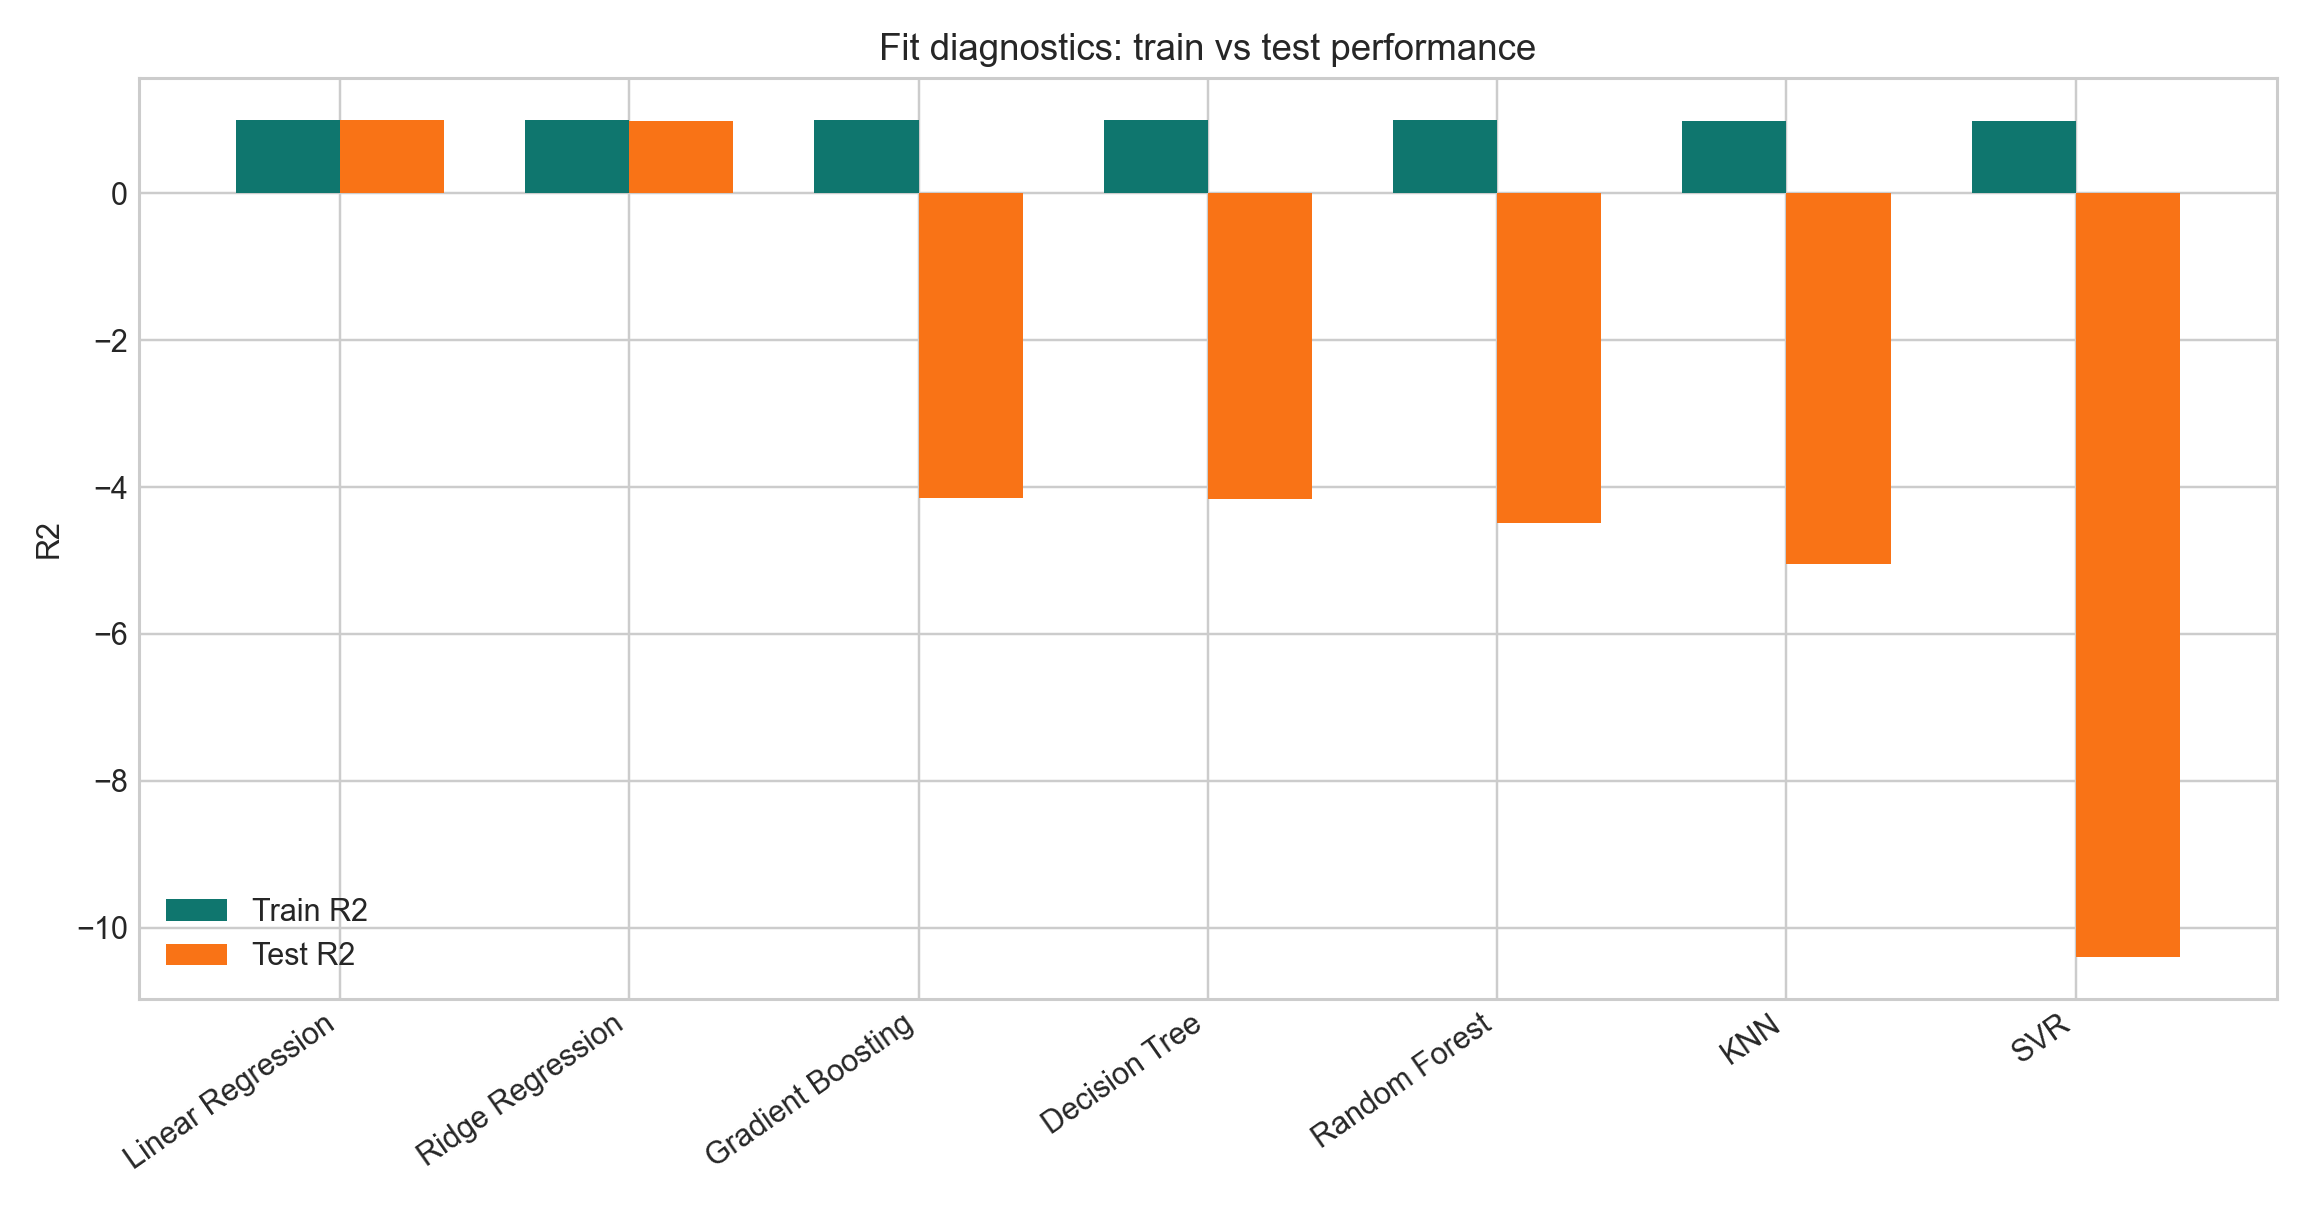
\includegraphics[width=0.92\textwidth]{figures/fit_diagnostics_results.png}
\caption{Fit diagnostics comparing train and test performance.}
\label{fig:generated_diag}
\end{figure}

The diagnostics figure shows whether a model generalizes beyond the training period. A large train-test gap indicates overfitting risk, while a weak score on both sets indicates underfitting. This is why the final project does not rely only on the highest raw score: it also asks whether the result is stable and explainable.

\begin{figure}[H]
\centering
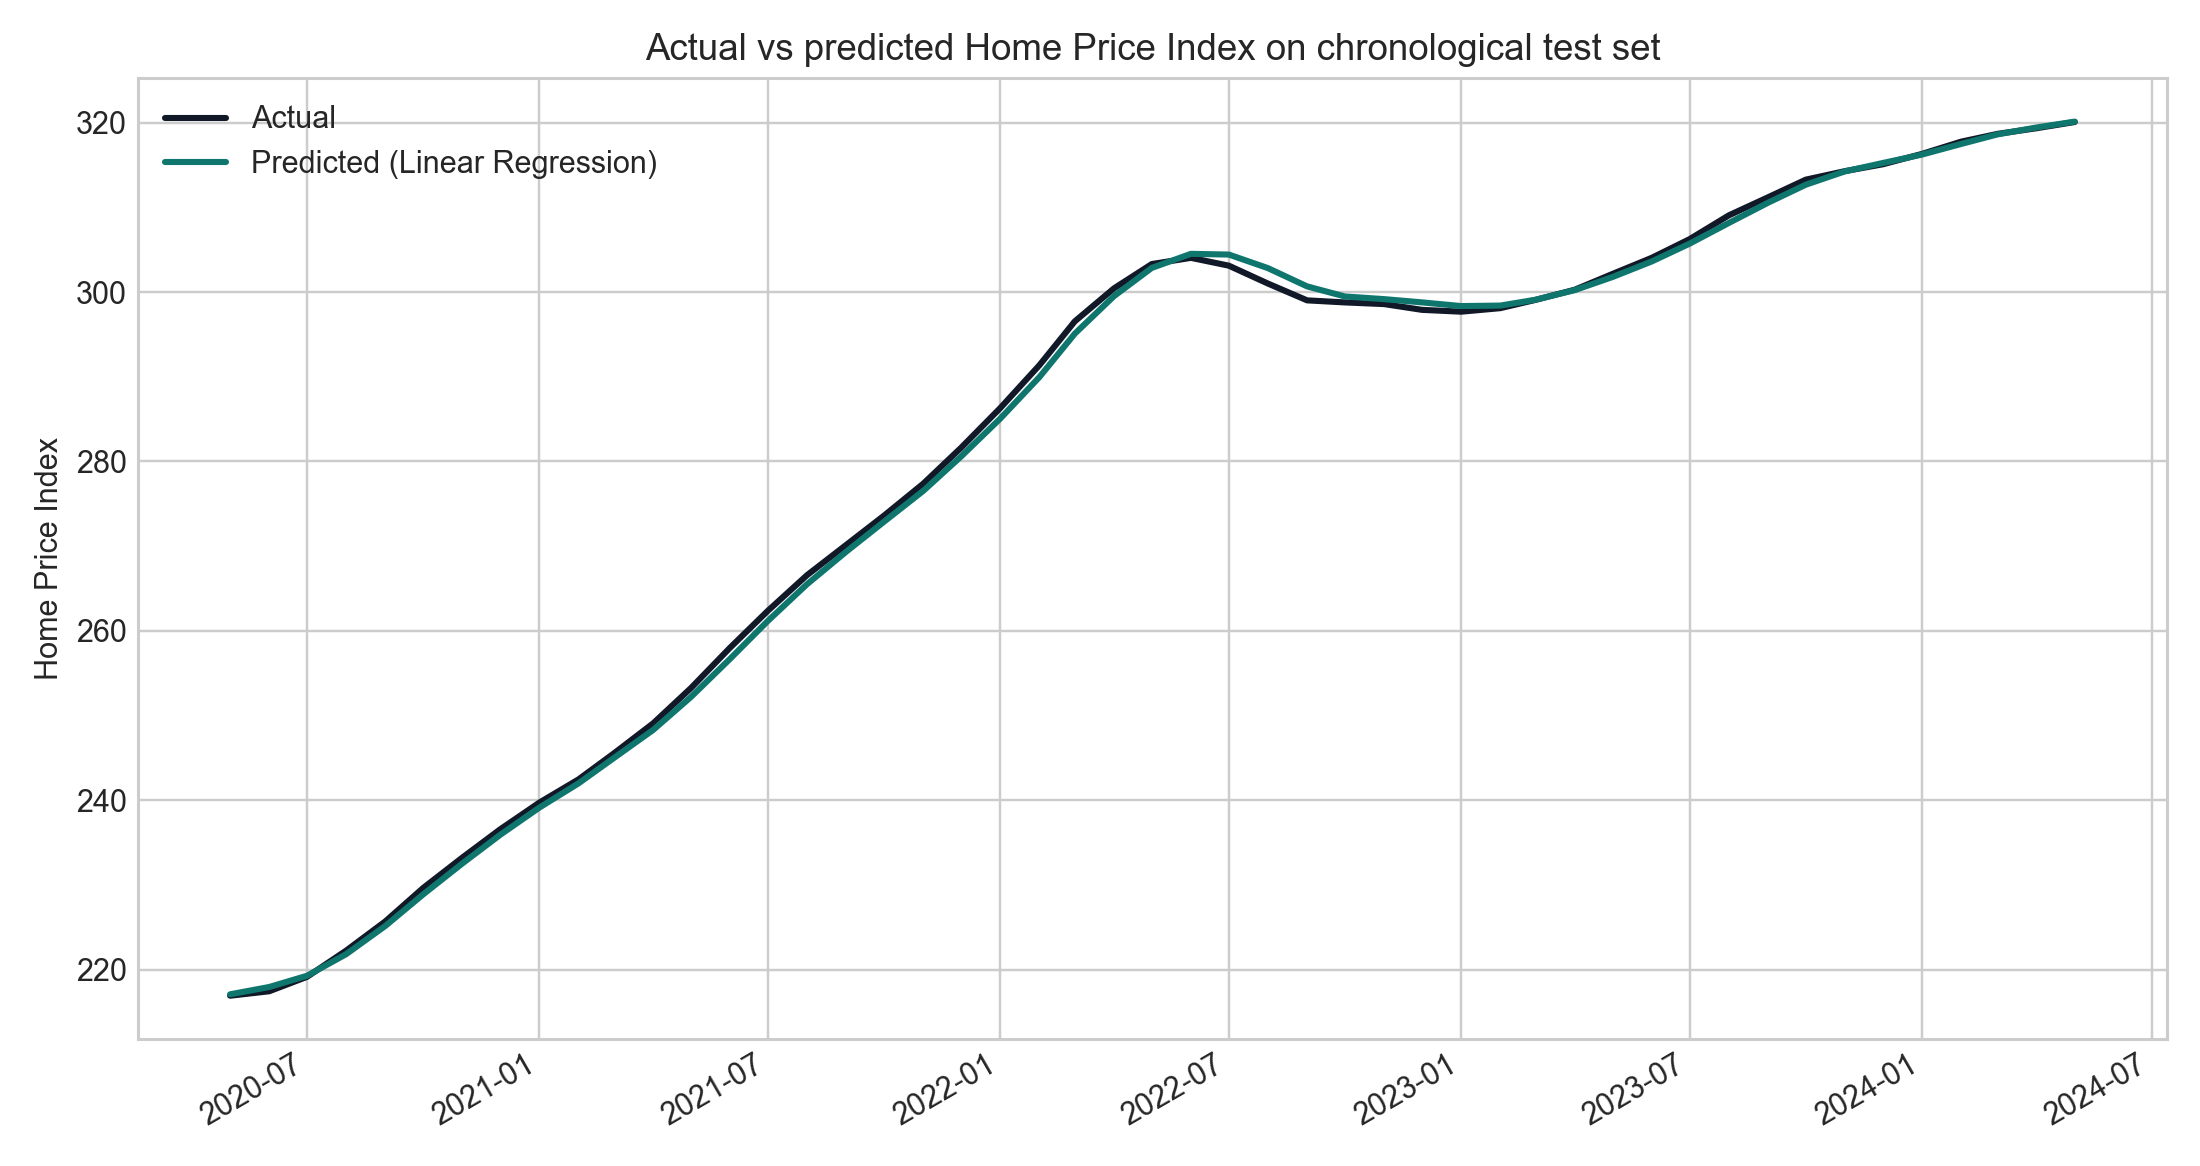
\includegraphics[width=0.92\textwidth]{figures/actual_vs_predicted_results.png}
\caption{Actual and predicted Home Price Index for the best model on the test period.}
\label{fig:generated_pred}
\end{figure}

\begin{figure}[H]
\centering
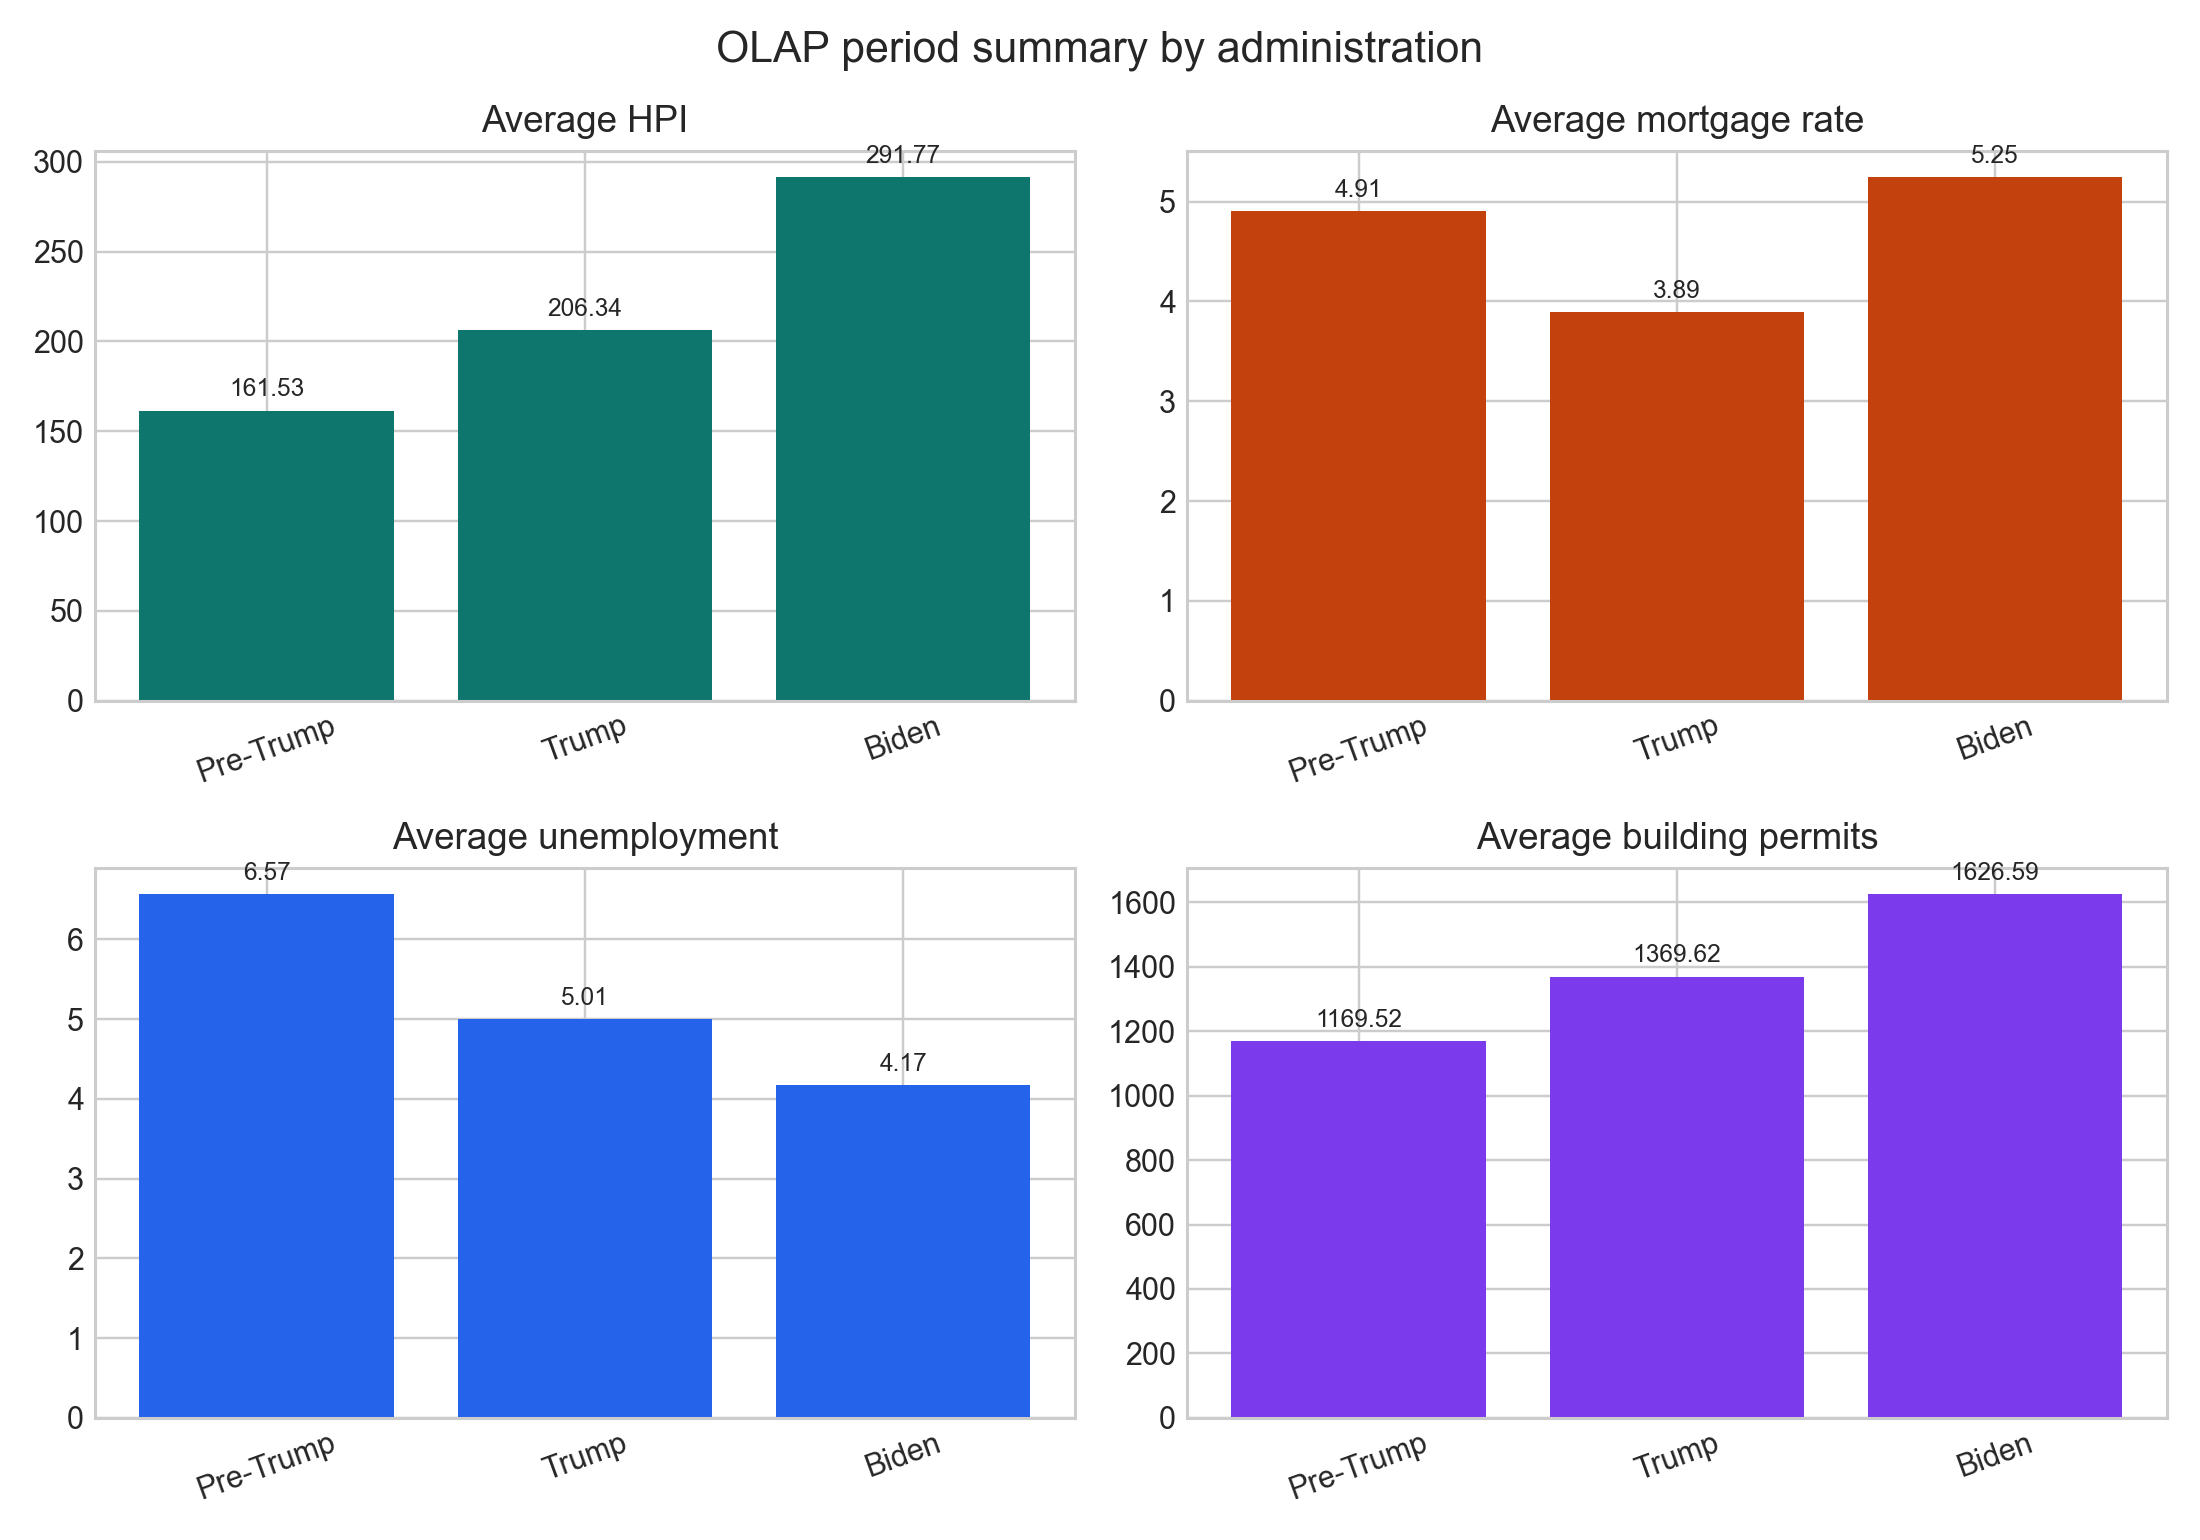
\includegraphics[width=0.95\textwidth]{figures/olap_period_results.png}
\caption{OLAP-style period comparison by administration.}
\label{fig:generated_olap}
\end{figure}

The OLAP summary shows that the highest average Home Price Index appears during the \textbf{Biden} period, while the highest average mortgage-rate pressure appears during the \textbf{Biden} period. This result is useful for the paper-review argument: prices and affordability pressure can rise together when supply, timing, and market inertia slow the response of prices.


\section{Limitations}

Despite the quality of the workflow, the project has several limitations.

First, the dataset may not capture all the determinants of housing prices.
Important factors such as regional heterogeneity, demographic evolution, or credit access variables may be absent.

Second, the forecasting logic is relatively simplified.
It uses a supervised learning strategy with lagged features rather than a dedicated time-series framework such as ARIMA, Prophet, or recurrent neural networks.

Third, the presented model results depend strongly on preprocessing decisions and the specific target selected by the user.
Different datasets or feature sets could lead to different outcomes.

\section{Recommendations and Future Improvements}

Several improvements can strengthen the project:
\begin{itemize}
\item integrate larger and more recent datasets,
\item include external APIs for automatic data refresh,
\item test advanced forecasting techniques,
\item improve the visual design of the dashboard,
\item add regional filtering or scenario analysis.
\end{itemize}

It would also be valuable to include a dedicated explainability module, for example with SHAP values, in order to deepen the interpretation of feature contributions.

\section{Conclusion}

This chapter discussed the most important results of the project.
The experiments showed that machine learning methods can provide useful insight into housing market dynamics and that Random Forest offers stronger predictive performance than Ridge Regression in the proposed setting.
At the same time, the dashboard contributed significantly to the interpretability and practical usability of the project.
Overall, the work confirms the relevance of data mining and machine learning for economic analysis and opens the door to more advanced future developments.

\section{Results from the Analytical Platform}

The platform produces a broad set of results that includes exploratory findings, Ridge Regression, Random Forest, forecasting, comparative model evaluation, unsupervised discovery, OLAP summaries, reinforcement-learning interpretation, paper review, production-readiness checks, and business impact analysis.

\section{Supervised Model Comparison}

The expanded model laboratory makes it possible to compare different algorithms on the same dataset and feature selection. This improves the reliability of the modeling decision. A model should not be selected only because it is popular; it should be selected because it performs well, remains interpretable enough for the context, and behaves consistently.

\begin{longtable}{p{4cm}p{5cm}p{5cm}}
\toprule
\textbf{Model family} & \textbf{Strength} & \textbf{Limitation} \\
\midrule
Linear Regression & Simple and interpretable & May underfit non-linear relationships. \\
Ridge Regression & Stable baseline with regularization & Still mainly linear. \\
Random Forest & Captures non-linear patterns and interactions & Less transparent than linear models. \\
Gradient Boosting & Often strong predictive accuracy & Requires careful tuning. \\
Decision Tree & Easy to visualize conceptually & Can overfit without constraints. \\
Support Vector Regression & Effective for complex boundaries & Sensitive to scaling and parameters. \\
KNN & Simple similarity-based logic & Can be weak in high dimensions. \\
Neural Network & Flexible function approximation & Requires more data and careful training. \\
\bottomrule
\caption{Interpretation of model families used in the platform.}
\end{longtable}

\section{Interpretation of Unsupervised Results}

The unsupervised learning results should be interpreted as exploratory findings. Clusters do not automatically represent economic truth; they identify similarity patterns according to selected features. If clusters align with known historical periods, this strengthens the interpretation. If clusters cut across periods, this suggests that macroeconomic profiles may be more complex than political labels alone.

PCA helps identify whether a small number of components explain much of the variation in the dataset. If the first two components explain a large share of the variance, visual analysis becomes more reliable. If the explained variance is low, the dataset is more complex and cannot be summarized easily in two dimensions.

Anomaly detection is particularly useful for housing-market analysis because abnormal periods can correspond to major economic shocks. These may include the financial crisis, pandemic-related disruptions, or high-rate affordability pressure.

\section{OLAP Results and Interpretation}

OLAP summaries provide a bridge between raw data and business understanding. For example, grouping indicators by administration period can reveal whether average mortgage rates, unemployment, inflation, or housing prices differed strongly across periods. Pivot tables can also show how indicators behave across time segments.

The strength of OLAP is that it is easy to explain. A manager or non-technical user can understand averages, medians, and period comparisons more easily than complex model internals. For this reason, OLAP results are useful before and after machine learning. Before modeling, they help understand the data. After modeling, they help interpret whether model results are coherent with descriptive patterns.

\section{AI Chatbot Results}

The chatbot improves the accessibility of the project. Instead of requiring users to navigate every technical page alone, the AI assistant can explain metrics, summarize outputs, and guide the user through the dashboard. This is especially valuable in an academic project because it demonstrates awareness of user experience.

The chatbot should be used carefully. It should explain results based on the available data and avoid presenting predictions as certainty. Good chatbot behavior must include cautious language, context, and explanation of limitations.

\section{Paper Review and Theory Comparison}

The paper review and comparison module adds academic depth. A project about housing prices should not only show charts and models; it should also discuss whether the findings are consistent with economic theory.

The main theoretical expectations are:
\begin{itemize}
\item higher mortgage or interest rates generally reduce affordability and pressure prices downward;
\item higher unemployment can weaken demand;
\item stronger income can support demand;
\item limited supply can keep prices high even when affordability worsens;
\item housing prices often react slowly because real estate markets are less liquid than financial markets.
\end{itemize}

The project therefore compares observed correlations and period changes with these expectations. When the dataset supports theory, the conclusion becomes stronger. When it challenges theory, the result is still useful because it may reveal timing effects, omitted variables, or mixed market forces.

\section{Real-Market Period Comparison}

The system compares the dataset with major housing-market periods:
\begin{itemize}
\item pre-crisis housing boom,
\item financial-crisis correction,
\item recovery and expansion,
\item pandemic-era demand shock,
\item high-rate affordability pressure.
\end{itemize}

This period comparison is important because housing-market behavior cannot be understood only through one global correlation. A variable may have one effect during a normal period and another effect during a crisis period. The project therefore interprets the housing market as a dynamic system.

\section{Production-Readiness Results}

The production-readiness module evaluates whether the data and model environment are reliable enough for serious use. It checks conditions such as dataset availability, duplicates, missingness, date column detection, and target variable availability.

The purpose of this module is not to claim that the academic project is already an industrial product. Instead, it shows what would be required to move toward professional deployment. This includes monitoring, documentation, validation, and governance.

\section{Business Impact}

The business impact of the project can be summarized in three levels.

\subsection{Analytical Impact}

The platform helps users understand which indicators are associated with housing prices, how these indicators change over time, and how models use them for prediction.

\subsection{Decision-Support Impact}

The dashboard supports what-if thinking, model comparison, and scenario interpretation. This can help analysts prepare reports, explain risks, or discuss possible market directions.

\subsection{Educational Impact}

The project is also valuable as a learning platform. It demonstrates how several data science concepts connect in one real application: EDA, supervised learning, unsupervised learning, forecasting, OLAP, reinforcement learning, AI interaction, and deployment.

\section{Limitations}

The project remains subject to several limitations.

\begin{itemize}
\item The dataset may not include all relevant housing-market determinants.
\item National-level data can hide regional differences between states and cities.
\item Forecasting is based on supervised lag features and does not replace specialized econometric forecasting.
\item The reinforcement-learning module is educational and simplified.
\item Chatbot answers depend on prompt quality and available context.
\item Streamlit deployment is practical but still needs security, authentication, and monitoring for professional production.
\end{itemize}

\section{Recommendations}

Future improvements should include:
\begin{enumerate}
\item adding regional housing datasets,
\item connecting live APIs for economic indicators,
\item adding SHAP explainability,
\item improving chatbot grounding with retrieved dashboard results,
\item adding user authentication,
\item saving experiment history in a database,
\item deploying the app on a cloud platform,
\item creating automatic PDF report generation,
\item and comparing results with more academic papers.
\end{enumerate}

\section{General Discussion}

The project shows that useful data science is not only about obtaining the highest score. It is about creating a coherent analytical workflow. A strong model without interpretation is difficult to trust. A beautiful dashboard without validation is risky. A chatbot without data grounding can be misleading. For this reason, the platform combines several layers: data quality, visualization, modeling, evaluation, explanation, deployment, and governance.

This combination makes the project more realistic and more valuable. It reflects how modern data science products are expected to work in professional contexts.

\section{Conclusion of the Results}

The results confirm the relevance of data mining and machine learning for housing-market analysis. The system now provides not only predictions but also segmentation, comparison, explanation, and interactive assistance. The project therefore forms a broader housing intelligence platform with academic, technical, and business value.
